\documentclass[12pt]{article}
\usepackage{hyperref}
\usepackage{hyperref}
\usepackage{graphicx}

\hypersetup{
    colorlinks=true,
    linkcolor=blue,
    filecolor=magenta,      
    urlcolor=cyan,
}
 
\urlstyle{same}
\title{CSE515T Status Report}
\author{Jesse Huang}

\begin{document}
\maketitle
\section{Progress}
I have obtained and cleaned the data provided by Bigquery.
My technology stack is Python with the Natural Learning Tool Kit,
and a LDA package. I am storing my data localling with SQLite3.  
Currently, I am working on getting this data into document-term matrix
form, so that I can feed it into LDA and LSA algorithms. 10 sample
'cleaned' comments are shown below:
\begin{center}
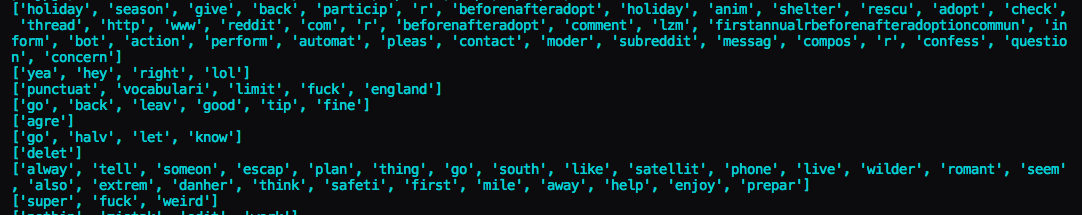
\includegraphics[scale=0.3]{sample-clean-data.png}\\
\end{center}
\section{Concerns}
The reddit comment database is broken up into separate datasets
by month. As such, I unsure how to sample uniformly from the
database as a whole. Currently, I have been randomly sampled 200
comments from each month, but feedback would be appreciated on
whether this is a solid choice to have made in building my local
dataset. This problem is further complicated by BigQuery's limit of 30TB/month 
of free processing, of which I have used roughly 40\%
\section{Pivots}
This limit has made my original proposal unfeasable, as to sample
comments from all of Reddit would use up my processing limit to obtain
relatively few samples.
Because of this limit, and the extremely wide range of topics
of the site as a whole, I have decided to focus on analysing the comments
from a single subreddit,
\href{https://www.reddit.com/r/confession/}{r/confession}. 
I believe this choice also helped mitigate some of the difficulties that
LDA has in modelling conversation, as most comments within
this specific subreddit are centered around responding to
confessions, as opposed to other comments. 
\section{Response to Feedback}
Thank you very much for the feedback that was provided for my initial report.
The questions posed are addressed below:
\textbf{\\Why is feature selection involved in topic modeling, say with LDA?\\}
It is not. I had initially proposed feature selection under with a misunderstanding
of topic models.\\
\textbf{How would I proceed to sentiment analysis based on topic modeling results?\\}
One method I was considering is to look at how the topic models
change overtime. However, I have not found much formal literature on
established ways to proceed with sentiment analysis through topic models, only
this somewhat informal \href{https://blog.insightdatascience.com/topic-modeling-and-sentiment-analysis-to-pinpoint-the-perfect-doctor-6a8fdd4a3904}{article}.
As such, suggestions as to how to proceed would be welcome.
\end{document}.